\documentclass[phd]{abdnthesis}

%% For citations, I would recommend natbib for its
%% flexibility, particularly when named citation styles are used, but
%% it also has useful features for plain and those of that ilk.
%% The natbib package gives you the following definitons
%% that extend the simple \cite:
%   \citet{key} ==>>                Jones et al. (1990)
%   \citet*{key} ==>>               Jones, Baker, and Smith (1990)
%   \citep{key} ==>>                (Jones et al., 1990)
%   \citep*{key} ==>>               (Jones, Baker, and Smith, 1990)
%   \citep[chap. 2]{key} ==>>       (Jones et al., 1990, chap. 2)
%   \citep[e.g.][]{key} ==>>        (e.g. Jones et al., 1990)
%   \citep[e.g.][p. 32]{key} ==>>   (e.g. Jones et al., p. 32)
%   \citeauthor{key} ==>>           Jones et al.
%   \citeauthor*{key} ==>>          Jones, Baker, and Smith
%   \citeyear{key} ==>>             1990

\usepackage{natbib}
%\usepackage[round,colon,authoryear]{natbib}
\setlength{\bibsep}{0pt}
\bibliographystyle{plain}
%\bibliographystyle{apalike}

\usepackage[T1]{fontenc}

\title{Summarizing online discussion with point extraction}
\author{Charlie Egan}
% IMO this is a bit silly, but some like to include these. To remove,
% delete this declaration and remove the option from the
% \documentclass definition above.
%\qualifications{PhD, Computer Science, University College London, 1997\\%
%BEng (Hons.) Electrical and Electronic Engineering, The University of Wales, Swansea, 1992}
\school{Department of Computing Science}

%%%% In the final submission of a thesis, this should only be the year
%%%% of submission.  However, it is useful to use \date{\today} for drafts so that
%%%% they don't get mixed up.

\date{2016}

%% It is useful to split the document up as chapters and include
%% them.  LaTeX will sort out all the numbering and cross-referencing
%% for you --- if you run it enough times!

%% If you want to include only a couple of chapters then use the
%% \includeonly{} command with a list of the file/chapter names that
%% you wish to include.  NB, this must be in the preamble.

\includeonly{introduction}

\def\sfthing#1#2{\def#1{\mbox{{\small\normalfont\sffamily #2}}}}

\sfthing{\PP}{P}
\sfthing{\FF}{F}

%% This will make sure that all cross-references are correct (including
%% references to those file not included) but will produce a dvi
%% file with only those files/chapters you specify included.

\begin{document}

%%%% Create the title page and standard declaration.

\maketitle
\makedeclaration

%%%% Then the abstract and acknowledgements

\begin{abstract}
  With an ever increasing number of internet users, online communities are hosting an increasingly large number of discussions. This user generated content contains millions of statements, opinions and ideas. Our systems for discovery of such information are playing catch-up and in the meantime much of this resource is lost.

  In this paper an approach for summarising such information is proposed. Our approach is based on the idea of `point extraction', where a point is a verb and it's associated arguments. We implement and test our approach on six online debates before evaluating our summaries against a baseline. We found that we were able to improve significantly on the baseline summaries of the same debate.
\end{abstract}

\begin{acknowledgements}
  \begin{itemize}
    \item{Adam \& Advaith}
    \item{Angrosh}
    \item{Parents}
    \item{Apple Store}
    \item{Department}
  \end{itemize}
\end{acknowledgements}

%%%% It should have a table of contents, but delete the other two as
%%%% necessary.

\tableofcontents
%\listoftables
%\listoffigures

\chapter{Introduction\label{chap:introduction}}
  More people are online than ever before. Comment threads and forums allow us to spend our spare time participating as contributors - rather than just consumers consumers. From the latest blockbuster title to yesterday's celebrity misdemeanor there's an online conversation already well underway.

  These discussions, where statements are encoded in natural language, represent a large untapped resource of ideas and opinions. A higher level view of this ever-evolving `data set' would be of interest to many working the social sciences as well as the participants of online discussions.

  This project explores an approach for summarization of such information. At the core of the approach is the notion of a `point' - a short refined argument statement. An argument is made up of a number of points and we are going to use these as our content units in our summarization task. Points are extracted from text and grouped to give a summary of the discussion. We test our implementation's performance by running an evaluation using summaries generated from various political debates sourced from online discussions \cite{walker2012corpus}.

  \section{Motivation}
    ``A summary can be loosely defined as a text that is produced from one or more texts, that conveys important information in the original text(s), and that is no longer than half of the original text(s) and usually significantly less than that.'' \cite{radev2002introduction}

    Summarization has been a long-running task in the field of Natural Language Processing. Summarization sub-tasks such as extraction and compression, where text is selected and removed to arrive at a summary, have become commonplace due to the complexities introduced by abstractive methods. Extractive methods for this have become largely statistical using Naive-Bayes \cite{kupiec1995trainable} approaches and, more recently, Neural Networks \cite{svore2007enhancing}.

    Argumentation Mining, a newer area of study, has the aim of detecting argumentative discourse structure in text. Argumentation Mining has been successfully used in the processing of formal texts such as parliamentary records \cite{palau2009argumentation} and legal documents (cite: Semantic Processing of Legal Texts) where arguments are often stated more explicitly. However, Argumentation Mining has also more recently been applied to more informal text \cite{park2015conditional}. Such applications, coupled with summarization, encapsulates much of the idea for this project.

    The points idea was adopted from a previous project from the department that used points in a system for stance classification. This had point identification, however, the tool was not capable of extracting units of text smaller than sentences. The tool was capable of linking contrasting points, but could only make matches based on the present of negation terms.

    The project was based on the concept of a point as well as the idea that informal argumentative discourse could be used to build a high-level summary of an online discussion. News article comment sections; forum threads; film \& product reviews and even extended email conversations are all candidate applications for such a tool.

  \section{Objectives}
    Starting with the definition for a point: a verb and it's dependents, we set the following objectives for the project.

    Leading on from the stance classification project (cite Angrosh?), we wanted to improve on the extraction of points from text. This meant ensuring a complete list of a verb's dependents was maintained for presentation for a given point - rather than just using the containing sentence.

    Another goal was to investigate relationships between points such as contrastive or co-occurring points - this involved expanding the ways in which related points could be matched, beyond negation. As secondary objective, we wanted to investigate supporting points. These were points that not only commonly co-occured in posts but also had a place in an argument structure.

    The task of stance classification was also discussed. Another secondary objective was to investigate if certain points were representative for a given known stance. Stance was annotated on some of the corpus debates.

    Finally we set out to present this information in in a way that was easy to interpret. This `presentation form' evolved into our debate summaries.

\chapter{Background \& Related Work\label{chap:background-related}}
  \section{Background}
    This project is built on existing technologies and research. This section gives an overview of the key foundations.

    \subsection{Automatic Summarization}
      ``A summary can be loosely defined as a text that is produced from one or more texts, that conveys important information in the original text(s), and that is no longer than half of the original text(s) and usually significantly less than that.'' \cite{radev2002introduction}

      Approaches to summarization could be grouped loosely into two groups, extractive and abstractive. Extractive summaries are constructed using content found in the source text. Abstractive summaries generate the summary content by performing some form of analysis on the source text. One might also group summarization tasks based on the nature of the source text. Approaches tend to summarize either single or multiple documents.

      This project is more closely related to the summarization of multiple documents, however, it applies both elements of extraction and abstraction.

      \subsubsection{Multi-document Summarization}
        Summarizing text made up of documents from different authors poses an interesting challenge. Using multiple documents introduces repetition and contradictions - this makes selection tasks such as extraction and compression more complex.

        Earlier work on multi-document summarization suggested the task was going to require an abstractive approach \cite{McKeown1999TMS315149315355}. The justification being that extraction techniques used for single document summaries, not being able to connect information between documents, would lead to incoherent and repetitive summaries. An alternative approach clustered paragraphs on the same topic from multiple documents and then use natural language generation techniques to combine phrases from paragraphs into a coherent summary \cite{McKeown1999TMS315149315355}. A similar approach creates clusters by parsing sentences and using predicate-argument structures to link phrases \cite{barzilay1999information} (comment about being similar to our points extraction and grouping?). Interestingly, while both rely methods rely on natural language generation, neither use a semantic representation.

        More recently, MEAD, a centroid-based, multi-document summarization tool has been able to produce good summaries without abstraction and generation \cite{radev2000centroid}. Compared to previous abstractive systems such as SUMMONS that relied on templates \cite{mckeown1995generating}, MEAD was more generally applicable.

        Most work on the summarization of multi-document sources has focused on news articles. While there are parallels between this and the summarization of online discussion, fundamentally they are different tasks. More closely related to this project is opinion mining.

        Opinion mining or sentiment analysis is an approach often applied to user reviews, documents discussing a product or service. Early work in the area focused on the problem as a classification task, categorizing documents based on their sentiment bearing terms \cite{turney2002thumbs}. More recently there as been a greater focus on aspect-based approaches that attempt isolate sentiment terminology to specific topics such as product features \cite{hu2004mining}.

      \subsubsection{Sentence Compression \& Content Unit Size}
        While sentences are often the default `content unit' used in extractive summarization, often smaller units are more desirable. Sentences found in real documents and discussions can make a number of statements each of which can be useful when creating a summary. Sentences may also include surplus information. In this case sentences can be compressed statistically, in a similar way to documents are in extractive summarization.

        Both noisy channel and decision based models have used on parsed sentences for the task of sentence compression \cite{knight2000statistics}. Our approach for compression where points are extracted around a verb, does not seem to have been previously documented.

        (comment that the largest coherent unit is a sentence in an extractive summary, even that might not be right (bad grammar, co-referring expressions). Reference: Ultra-Summarization: A Statistical Approach to Generating
        Highly Condensed Non-Extractive Summaries)

      \subsubsection{Evaluation of Summaries}
        The evaluation of automatically generated summaries is an ongoing discussion. A common approach is to make a comparison against a model summary, typically written by a human. Various metrics such as ROUGE \cite{lin2004rouge} are used to make the comparison between summaries statistically. These are however limited by the assumption that there is a single best model for a summary. Alternative methods have been proposed. The Pyramid Method is one such example, it models content units across the collection of summaries being evaluated to give each content unit a weight based on how commonly it occurs \cite{nenkova2004evaluating}. These weights are used to allocate scores to summaries without an ordering bias.

        Automated methods are used primarily at the Document Understanding Conference when many summaries must be evaluated for a given task. Ideally however summaries could be manually evaluated. This would allow extrinsic attributes such as the utility of a summary for a particular task to also be accounted for. (reference to SUMMAC?, automated http://citeseerx.ist.psu.edu/viewdoc/summary?doi=10.1.1.13.489)

        In this project we compare our summaries against those generated using the approach outlined here \cite{nenkova2006compositional} as a baseline.

    \subsection{Argumentation Mining}
      Argumentation Mining is a task that involves the identification components of arguments within text such as premises and the conclusion. The task also often involves fitting these components into a template or known pattern to enable some form of reasoning. \cite{palau2009argumentation}

      A relatively new research area - combining ideas from natural language processing, information extraction and argumentation theory - argumentation mining is based largely on discourse  theory. While argumentation mining can be applied to structured text (source?), ultimately mining of free text is the goal. This means that argumentation tools often need to model concepts from linguistic research such as rhetoric structure theory \cite{mann1988rhetorical} and local coherence centering \cite{weinstein21centering}.

      \subsubsection{Identifying Argumentative Structures in Text}
        When identifying argumentative structures in text the first step is often to classify phrases that are part of an argument being made. One of option is to define rules for argumentative sentences or clauses. This can also be approached as a classification task, statistical methods such naive-bayes have also been used \cite{palau2009argumentation}. The result of this stage is a collection of unrelated clauses potentially spanning many arguments present in the source text.

        The next stage in the analysis is to group identified units together into separate arguments. While sometimes the document's structure (chapters and sections) can be used to inform the grouping task this is hard to make generally applicable. Documents are rarely consistently formatted and arguments will often span many sections. Other options include grouping based on the similarity of the unit contents - presence of certain words etc. \cite{palau2009argumentation}

        Once identified units have been grouped into different arguments it becomes possible to start looking into the argument's structure. Different units need to be classified as either premises or conclusions - this can again be approached as a classification task \cite{palau2009argumentation}. Once such as structure for the units has been established it's possible to do analysis this connected structure such as identifying supporting claims for conclusions.

        A further task is relating arguments within the document to one another, this is a far more challenging task. Fitting the argument structure to allowed patterns defined by a context-free grammar is one proposed approach \cite{palau2009argumentation}.

    \subsection{Dependencies}
      The approach implemented as part of this project relies on the products of research in the following areas.
      \subsubsection{Topic Modeling}
        Topic modeling covers a set statistical modeling techniques used to identify and group `topics' in text. Fundamentally, this involves looking for words that are relatively more common on one document vs a more general corpus. Documents often contain multiple topic words that need to be grouped into more conceptual topics. One approach to this is is Latent Dirichlet Allocation (LDA), this implements a "three-level hierarchical Bayesian model" \cite{blei2003latent} and is the approach used for topic modeling in this project.
      \subsubsection{Dependency Parsers}
        Parsing text for dependencies involves building upon a phrasal parse to extract relations between tokens in text. Dependencies are identified using rules applied to phrase structure trees. Various dependency parsers exist, this project makes use of the dependency parser included as part of the Stanford CoreNLP framework \cite{de2006generating} which is based on their probabilistic context-free grammar phrasal parser \cite{klein2003accurate}. The rules used in the Stanford dependency parser based on ``Universal Stanford Dependencies" \cite{de2014universal}.
      \subsubsection{Querying Dependency Parses}
        To make use of the dependency parse a means of querying the graph is required. \textit{Semgrex} is one such approach, this defines a regular expression style syntax for expressing queries on nodes and relations in a dependency graphs \cite{Chambers2007}. More generally however, the task about querying nodes and edges in a directional graph. For this project we opted to use \textit{Cypher}\footnote{http://neo4j.com/docs/stable/cypher-introduction.html}, the graph query language implemented by the \textit{Neo4j}\footnote{http://neo4j.com/} graph database. This was chosen for the querying of dependency parses because it allowed many separate graphs to be queried in parallel for the same pattern using a more familiar declarative syntax.

  \section{Related Work}
    Having covered the technologies and areas of research that underpin this project I will now discuss similar work that come closer to combining these different areas, as this this project does.

    Summarizing discussions, email and meetings

    Summarizing online and archived discussions

    Summarizing opinions on online discussions

    Argumentation in online discussions

    Argumentation driven summaries not been covered. (Result of the review of related work is that:  there does not appear to have been any work that approaches the summarization of discussion from an argumentation mining perspective.)

  \section{Motivation}
    Round up why our project is different and interesting

\chapter{Requirements\label{chap:requirements}}
  The functional requirements listed are only part of the evaluation for the project's success. The results of the evaluation where we test quality of the output as are also a key consideration.
  \section{Functional Requirements}
    To be elaborated
    \begin{itemize}
      \item{Extraction of points from raw text.}
      \item{All dependencies of the verb are correctly extracted as part of the point}
      \item{A clustering mechanism for identifying contrastive points}
      \item{An interface to inspect the content of a discussion}
    \end{itemize}
  \section{Non-functional Requirements}
    To be elaborated
    \begin{itemize}
      \item{Implement independent components to enable reuse in the analysis pipeline}
      \item{Capable of handling large discussions}
      \item{Use standard data formats for communication between pipeline components}
    \end{itemize}

\include{problem-domain}
\include{methodology-tech}
\include{system-design}
\include{testing}
\chapter{Evaluation\label{chap:evaluation}}
  This chapter will detail the evaluation metrics, how they were tested and what the results of the evaluation were. Two (or three) sets of evaluations were carried out making use of six debates from our corpus \cite{walker2012corpus}: abortion, creation, gay rights, the existence of god, gun ownership and healthcare.

  \section{Research Questions}
    We wanted to evaluate our tool as a tool for automated summarization. The result of a final analysis was a summary comprising of point extracts for a given debate, by assessing the quality of this we also evaluate the precursor analysis. The following research questions were set:

    \begin{itemize}
      \item{Are our summaries more readable and informative than those produced by existing tools?}
      \item{Does introducing summary sections with an explanation improve readability?}
      \item{What is the level of agreement between our extract selection module and humans given the same task?}
      \item{TBD: Which sections of generated summaries are most useful to readers?}
    \end{itemize}

    To address these questions we compared different versions of our summaries against equal-length summaries generated by an implementation of \cite{nenkova2006compositional} (`stock summaries'). We also gathered scores for groups of extracts and compared summaries generated with randomly selected extracts against one based on our bigram model for selection.

  \section{Design}
    In response to the our research questions we set the following null hypotheses for the evaluation:

    \begin{itemize}
      \item{The readability and informativeness of our summaries do not improve on those of existing tools. (\textbf{H1})}
      \item{Explanations introducing summary sections does not improve readability. (\textbf{H2})}
      \item{Our means of selecting extracts is not better than random selection. (\textbf{H3})}
      \item{\textcolor{red}{TBD: All summary sections are equally useful to readers. (\textbf{H4})}}
    \end{itemize}

    To test these hypotheses we prepared three comparative studies. These are described in the following sections.

    \tocless\subsection{Summary Styles}
      In the upcoming sections, reference is made to a range of summary styles.
      \begin{itemize}
        \item{\textbf{Stock}: A summary generated using an implementation of \cite{nenkova2006compositional}, used as a benchmark for summaries generated by our tool. There is no structure to these summaries.}
        \item{\textbf{Plain}: This is a collection of point extracts in the same styles as the stock summaries. The order of extracts is the same as it would be if the summary had sections annotated. This presentation is designed to be as close as possible to the stock summary presentation.}
        \item{\textbf{Layout}: A summary that has explanatory text that introduces sections. The extracts are the same as those in the plain summary.}
        \item{\textbf{Formatted}: A layout summary with explanation keywords in bold and topic words in green.}
      \end{itemize}

      Participants for Study 1 and 2 were recruited using Amazon Mechanical Turk. \textcolor{red}{In the third study\dots}

    \tocless\subsection{Study 1: Summary Comparison}
      In order to address \textbf{H1} and \textbf{H2} we designed a questionnaire that compared various summary styles against equal-length stock summaries. Each questionnaire was made up of three sections.

      The first section compared a plain summary against a stock summary, on the same topic. Users were instructed to read both summaries and rate them relatively on the following criteria: `Content Interest / Informativeness', `Readability', `Punctuation \& Presentation' and `Organization'. Finally they they were asked to give an overall rating and justify their response. The next section asked the same questions but instead compared a layout summary against a stock one. Layout summaries are longer because of the explanatory text, the stock summary was the same length as the layout summary and was longer than the stock summary used in the first section. The final section compared a layout summary with a formatted one. The layout summary is reused from the second section, the formatted summary is also the same content (only different formatting). There was only an overall rating and justification for the comparison in this section.

      There were six versions of the questionnaire setup in a Latin square to cover all six topics. Section 1 had a different topic from sections 2 so as to not repeat summary content. Section 3 addresses the question of formatting only and has the same content as the layout summary in section 2 to make the task faster.

      Responses from the first section that compare our plain summary against a stock one can be used in addressing \textbf{H1}. The difference in the responses gathered in section 2 will allow us to address \textbf{H2}. Section 3 extends on this, testing if the formatting is a useful addition to the layout summary.

    \tocless\subsection{Study 2: Extract Comparison}
      To investigate the performance of the tool in greater depth we ran a further study testing the quality of our extract selection mechanism. Responses from this questionnaire addressed \textbf{H3}.

      The task given to participants had two sections. First were a series of extracts for a number of point patterns, participants were asked to rate extracts accounting for their succinctness and the extent to which they made sense. This was the closest we could make the task for participants to that of the tool. The following section, similar to the first study compared two summaries. Both summaries were of the formatted style however their content differed. The extracts in one summary were selected using the bigram model, the extracts in the other were selected at random. Participants were asked to give these a relative rating and justify their response. Responses for these two tasks were both intended to address \textbf{H3}.

    \tocless\subsection{\textcolor{red}{TBD: Study 3: Section Comparison}}

  \section{Results}
    \subsection{Study 1: Summary Comparison}
      The results of the summary comparison showed a strong preference for summaries based on points based extraction. When comparing the plain and stock summaries, our plain summaries were marked as better or much better by 69\% of participants. Plain summaries, lacking any kind of layout, was still scored better or much better by 57\% of participants.

      When comparing layout summaries against equal length stock summaries participant preference only became clearer. 89\% of participants rated layout as better or much better than stock. Organization saw the greatest change, with a 30\% increase in favor of layout summaries. The average increase across all factors was 19\%. The ratio of `better' to `much better' also shifted, `much better' ratings increased by 15\% while `better' ones decreased by 5\%.

      There was also variation between summaries of different discussions. The gay rights layout summary saw an increase of 45\% in better/much better scores while the guns layout summary saw no improvement. When comparing plain and stock summaries on guns and healthcare all participants rated plain as being the same or better. When comparing the healthcare layout and stock summaries all participants marked the layout summary as being much more readable. The plain vs stock creation summary was the most divided, 42\% of responses were marked as same or stock better.

      Despite the points used in the layout and plain summaries being the same, the `Content' factor saw an increase of 14\% in better/much better scores. Punctuation was also saw a 13\% increase, despite also being the same.

      Regarding the results of the layout / formatted summary comparison, more than half of respondents preferred the formatted version of the summary. This is significantly lower than the improvements of layout vs stock (89\%) or even plain vs stock (69\%).

      These findings are based on the 55 responses from 6 different questionnaires giving 165 summary comparisons, the target population being people interested in online discussions.

      To test the significance of these results we use one-sided Sign test for matched pairs. Neutral responses were excluded, better \& much better responses were amalgamated. When comparing plain against stock, 38 successes in 45 trials, we found the probability for success is not equal with $p << 0.01$ (\textbf{H1}). Comparing layout and stock summaries, 49/53, we found that success is also not equal, $p << 0.01$. However, when comparing the layout and formatted summaries, 29/41, we found $p = 0.16$ and thus unsuitable to reject the null hypothesis at this level. These results are based on all responses across the different topics.

      (need to show that the layout improves on the plain vs stock, not sure how adjust my data to a Friedman Rank Sum Test)

      To conclude, the results show a preference for points based summaries. This can further be improved by introducing sections (if I can show statistical significance?). However we cannot say decisively that our formatted summaries improve on our layout versions.

    \subsection{Study 2: Extract Comparison}
      Our second study also gave a clear result. Extracts selected by our tool for display were scored above the user's mean score 74\% of the time. Selected extracts scored 3.94/5 on average while extracts not selected scored 3.11/5.

      (Results of a Mann-Whitney U test, or some other means of comparing the selected vs not extracts regarding the values from the likert scale scores. This is quite hard\dots)

      Currently results of a MWU test would read (where A is selected and B is not selected by the tool): The medians of Group A and Group B were 5 and 3, respectively. We ran a Mann-Whitney's U test to evaluate the difference in the responses of our 5-Likert scale question. We found a significant effect of Group (The mean ranks of Group A and Group B were 1026 and 767, respectively; U = *155681*, Z = *7.045*, p= 1.851 * 10\^-12, r = 0.0.17).

      \begin{figure}[h]
        \caption{\textcolor{red}{SAMPLE PLOT, machine z scores vs z scores of \textit{mean} human ratings}}
        \centering
        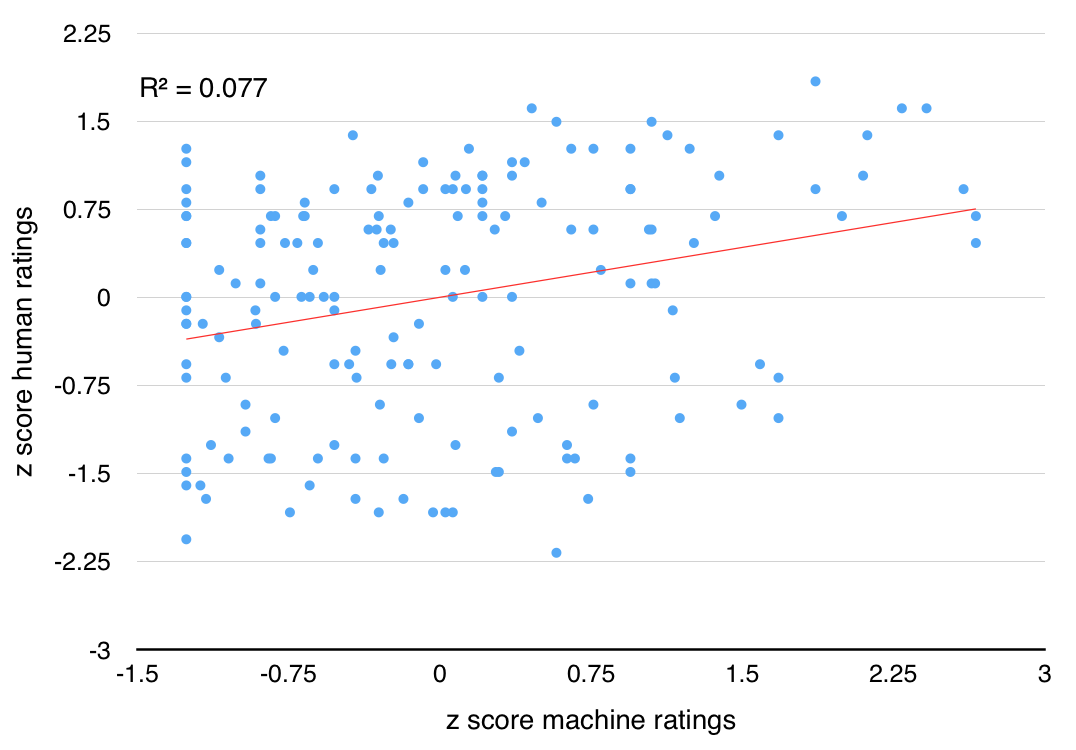
\includegraphics[width=0.8\textwidth]{extract_z_scores}
      \end{figure}

      Or the results can be presented like this:
      \begin{figure}[h]
        \caption{\textcolor{red}{group the human scores 1-5, then for each score plot the corresponding machine score in the box plot}}
        \centering
        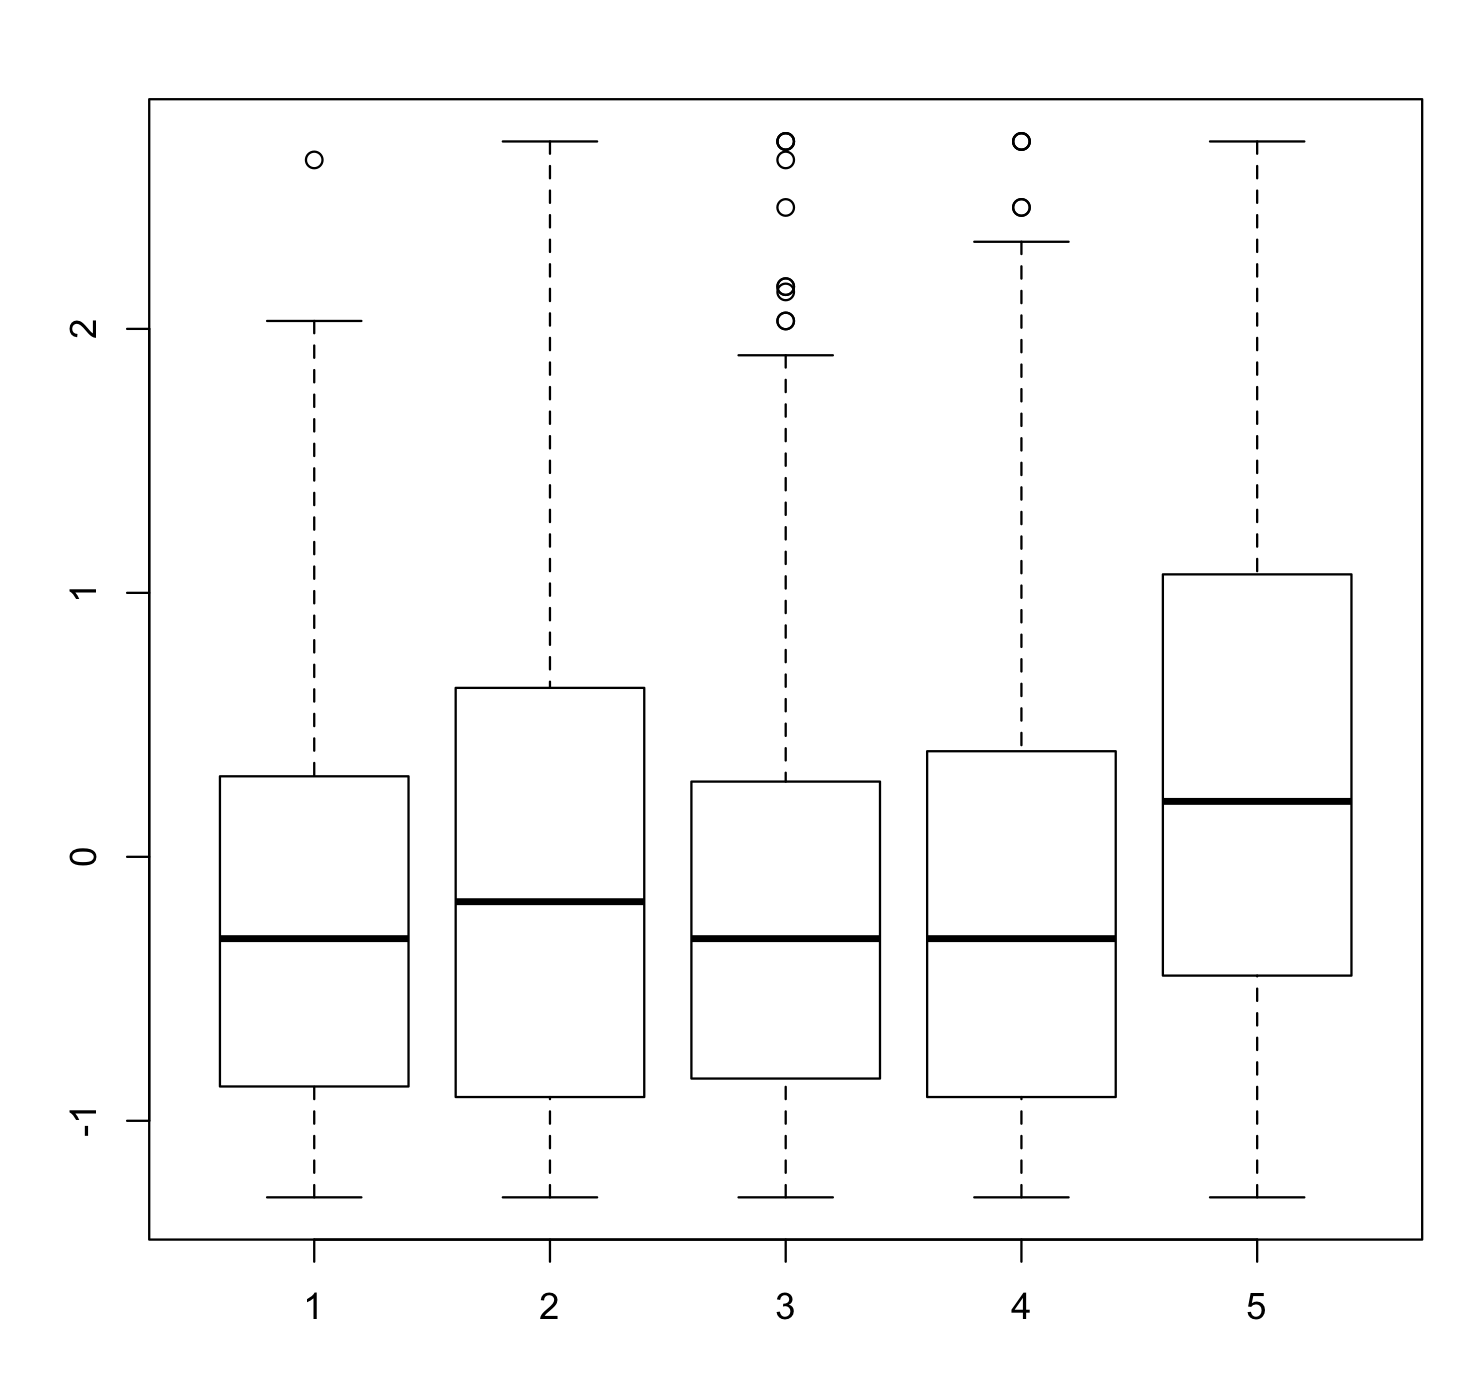
\includegraphics[width=0.8\textwidth]{boxplots}
      \end{figure}

      One selected extract \blockquote{As they pay income taxes} scored particularly poorly with a score of mean score of 2.2/5. Generally ratings correlate with the extract quality. These results are based on 1587 responses for 18 different clusters of extracts from six topics. The target population of this sample is all clusters of extracts selected for display in summaries.

      Regarding the results of the bigram vs. random summary comparison, there appeared was a preference for the bigram summary. 43\% of participants preferred the bigram summary, 20\% scored them the same and 34\% preferred the randomly generated summaries. Breaking this down by topic, the abortion bigram summary scored more than 5 times the random summary; for creation and healthcare both summaries scored equally. Interestingly, the random god summary scored higher than the accompanying bigram one.

      To test these results against \textbf{H3} we again used a one-sided Sign test. Excluding neutral ratings, the bigram model was successful 24/44 times. Based on this result we are unable to reject \textbf{H4}.

    \subsection{\textcolor{red}{TBD: Study 3: Section Comparison}}

  \section{Discussion}
    Based on on comments left as justification, some found the colors distracting and unnecessary as well as making the summary noisy and hard to read.
    Also need some samples of the comments that highlight interesting things

    On average, extracts scored well, showing pre-filtering is good at it's job.


    "Side [RANDOM] uses the scientific method and doesn't involve a fake diety at all in the science section." why god rand was better (also sentences made more sense)

\chapter{Summary \& Conclusion \label{chap:conclusion}}
  \section{Summary}
    In this project we have implemented a robust method for extracting points, a meaningfully shorter content unit than sentences. We make use of these in a summarization task by clustering points into cohesive sections. We then evaluate the effectiveness of our approach by comparing our summaries against those generated by a baseline statistical tool that uses sentence extraction.

    We were able to meet most of the project's initial goals. Using dependency parses, we have implemented a means of extracting more useful and complete points than those in previous project. We also improved on the detection of counter points by expanding the approach to account for antonyms --- rather than using negation terminology alone. While we also implemented an approach for the identification of co-occurring points, the results seem to be more variable and are highly dependent on large discussions where participants make many points.

    We opted to present the results of the analysis as summaries of the debate. Here we were able to go beyond our goals of counter/co-occurring points and include additional sections based on the points we had extracted. There are however areas that require further work. Results from our evaluation suggest that certain presentation decisions we not always popular. We also found that while scores allocated my our bigram model correlated with those of participants, this approach in selecting extracts from clusters was not significantly better than random when a compared at the summary level.

    The results of the summary comparisons were very positive with all our summary types performing significantly better in comparisons. We were able to reject our first two hypotheses. We were not able to reject \textbf{H3} but have gathered useful information for future work. We were unable to gather enough targeted feedback regarding sections to reject \textbf{H4} but again gathered much useful information for improving on the tool.

    Comments from study 3, at the social media workshop, suggested that the summaries fell between quantitative and qualitative analysis and this they could be made more useful by quoting the (already available) ratio of counter-point sides. Comments also suggested it would be useful to select the required summary length as well as provide links back to the input text. The disagreement section was referenced as being the most useful while participants found related points confusing.

  \section{Further Work}
    The implementation is still the product of an experimental development process. The components of the summary generation approach have poor maintainability. Next steps include reducing the agglomerative complexity and repetition as well as establishing a level of unit testing. Clearer definitions for the re-formatting of extracts and extract selection would also be beneficial for code readability. This ties into the corpus pre-processing and extract presentation, both areas that require a more integrated implementation.

    The tool chain is currently closely coupled with the corpus. We would like to establish a more less bespoke approach to make analysis of new corpora easier. One interesting direction would be a simple web application that capable of generating a summary for a discussion of the user's choosing from \textit{Reddit}, \textit{Hacker News} or online forum. This potential use case raises issue of the required discussion length. Currently a long discussion (upwards of 100,000 words) is required to extract a sufficient number of points to fill all our summary sections without repetition --- and build a good sample of counter/co-occurring points. This would likely require the summary structure to be more flexible, generating shorter summaries for shorter discussions and contextually removing sections where information was lacking.

    From the evaluation results we found that our bigram extract selection approach was not providing reliably better results than random --- though it's scores correlated with those of participants. This appeared to come down to both readability and informativeness. Currently extracts are weighted by the length, this is perhaps dominating the bigram score representing informativeness. It would also be interesting to introduce readability as an additional factor, perhaps by incorporating an \textit{Automated readability index}. Should the tool be made accessible to the public as a web application, there would also be the opportunity to use user rating of extracts to train a model for extract preference. The task of selecting readable, informative extracts that represent the cluster is an interesting task with various options for further work.

    Currently the approach models discussions as a flat list of posts --- without reply/response annotations. Using hierarchical discussion threads opens up interesting opportunities for Argument Mining using points extraction as a basis. A new summary section that listed points commonly made in response to other points in other posts would be an interesting addition. This would also be possible with discussions on \textit{Twitter} where reply information is also available. Related to this, adding user identity information would also make it possible to track a posts by the same user in discussions, and represents another interesting area for further features.

    Another direction that would be inserting to explore would be to build a graph-like representation of the discussion. Using point's subject and object information, a graph of nodes representing nouns connected by verbs as edges could be generated. This would be made more interesting if the semantic annotations from the verb frames could be included. As part of this project we experimented with a presentation of this type, an example is included in Appendix \ref{app:disc_graph}. Related to this is the possibility of using the semantic annotations in point frames to to investigate deeper abstractive summarization.

    There is also potential for further work on the summary presentation. Feedback gathered in Study 3 suggested that it would be useful to present the counts for negated points. This would allow the section to not only show a difference in opinion but to present how opinion is split. One comment suggested that the output was in between a quantitative and qualitative report and that adding more quantitative information to the summaries would make them more useful. Workshop attendees also suggested that being able to refer back to source text from the extracted points would also make the results more useful.

  \section{Conclusion}
    In this project we have shown that our points extraction is a viable foundation for summarization of online discussion. We think this success can be generalized to tasks beyond summarization that make use of text extracts. We have shown that existing tools struggle with the summarization of discursive text, and that our summaries with sections that are designed to give a more complete overview are preferred. Summarization is just one use case for such analysis and there are many other varied layers that could be built on top of our points extraction implementation.

    We see this project a step forward in the process of better understanding online discussion. Our hope is that this work can become the basis for further work and applications that allow the exploration of the wealth of ideas and arguments currently hidden in archived threads.


\appendix
\include{proof}

\bibliography{mybib}

\end{document}
